
\newif\ifTODO\TODOtrue                        % Use todo notes?

%===============%                               %~~~~~~~~~~~~~~~~~~~~~~~~~~~~~~~~~~~~~~~~~~~~~~~~~%
% DOCUMENTCLASS %                                See full option description in "mytemplate.cls"
%===============%                               %~~~~~~~~~~~~~~~~~~~~~~~~~~~~~~~~~~~~~~~~~~~~~~~~~%
 
\documentclass[
a4paper,10pt
]{ica2013_2}

\usepackage[utf8x]{inputenc}
\usepackage[table,dvipsnames,svgnames]{xcolor}
\usepackage{titlesec}

\newcommand\Fig[1]{Fig. \ref{#1}}

\newcommand\Grey[1]{{\color{Grey}#1}}
\newcommand\Red[1]{{\color{Red}#1}}
\newcommand\Blue[1]{{\color{Blue}#1}}
\newcommand\DarkBlue[1]{{\color{DarkBlue}#1}}
\newcommand\LightBlue[1]{{\color{LightBlue}#1}}
\newcommand\Brown[1]{{\color{Brown}#1}}
\newcommand\Green[1]{{\color{Green}#1}}
\newcommand\SeaGreen[1]{{\color{SeaGreen}#1}}
\newcommand\Yellow[1]{{\color{yellow}#1}}
\newcommand\Orange[1]{{\color{orange}#1}}

\ifTODO
   \newcounter{todoidx}
   \definecolor{todobackground}{rgb}{0.95,0.95,0.95}
   \setlength\marginparsep{1pt}
   \setlength\marginparwidth{35pt}
   \newlength\marginparwidthsmall
   \setlength\marginparwidthsmall{\marginparwidth}
   \addtolength\marginparwidthsmall{-7pt}
   \newcommand\todo[1]{%
      \addtocounter{todoidx}{1}%
      {\color{Red}\bf(\thetodoidx{})}%%\fbox{\bf\thetodoidx{}}}%
      \marginpar{%
         {\vspace*{-10pt}\color{Red}\fbox{\bf\thetodoidx{}}}\\%
         \fcolorbox{red}{todobackground}{\parbox{\marginparwidthsmall}{\scriptsize #1}}}}

   \newcommand\todopar[1]{\fcolorbox{red}{white}{\parbox{0.97\linewidth}{#1}}}
\else
%    \usepackage[disable]{./todonotes} 
   \newcommand\todo[1]{}
\fi

\newcommand\nn{\nonumber\\}

\newcommand\nmat[1]{\begin{matrix}#1\end{matrix}}
\newcommand\bmat[1]{\begin{bmatrix}#1\end{bmatrix}}
\newcommand\case[1]{\begin{cases}#1\end{cases}}
\newcommand\textbox[2]{\footnotesize\text{\parbox{#1}{\centering\emph{#2}}}}

\newcommand\rand{\text{rand}}
\newcommand\randn{\text{randn}}
\newcommand\rect{\text{rect}}
\newcommand\sinc{\text{sinc}}
\newcommand\tr{\text{tr}}
\newcommand\adj{\text{adj}}

% \newcommand\max{\text{max}}
\newcommand\argmin[1]{\text{arg}\,\underset{#1}{\text{min}}}

\newcommand\qqquad{\quad\qquad}
\newcommand\qqqquad{\qquad\qquad}

\renewcommand\l[1]{\left#1}
\renewcommand\r[1]{\right#1}

% {\text{\parbox{1.5cm}{\centering volume hyper- sphere}}}

%Keyword colouring:
\newcommand\kw[1]{#1}
\newcommand\parm[1]{#1}%\color{Black}#1\color{Black}}

\newcommand\of[1]{\scriptstyle(\parm{#1})\displaystyle}
\newcommand\df[1]{\scriptstyle[\parm{#1}]\displaystyle}
\newcommand\var[3]{#1_\text{#2}\of{#3}}

\newcommand\diag{\text{diag}}

% \raisebox{lift}[extend-above-baseline][extend-below-baseline]{text}
\newcommand\mt[1]{\text{\emph{#1}}} %mt = mathtext
\newcommand\mathnorm{\textstyle}
\newcommand\mathbig[1]{\displaystyle#1\mathnorm}
\newcommand\mathsmall[1]{\scriptstyle#1\mathnorm}
\newcommand\mathtiny[1]{\scriptscriptstyle#1\mathnorm}
\newcommand\sfrac[2]{\scriptstyle\raisebox{0.25pt}[0pt][0pt]{$\frac{#1}{#2}$}\mathnorm}
\newcommand\nfrac[2]{\textstyle\frac{#1}{#2}\displaystyle}

\newcommand\sumu[1]{\sum\limits^{#1}\,}
\newcommand\suml[1]{\sum\limits_{#1}\,}
\newcommand\sumb[2]{\sum\limits_{#1}^{#2}\,}

\newcommand\produ[1]{\prod\limits^{#1}\,}
\newcommand\prodl[1]{\prod\limits_{#1}\,}
\newcommand\prodb[2]{\prod\limits_{#1}^{#2}\,}

\newcommand\defeq{\overset{\underset{\mathrm{def}}{}}{=}}

%Math macros:
\newcommand\diff[2]{\frac{\kw{d}\,\textstyle #1\scriptstyle}{\kw{d\parm{#2}}}\displaystyle}
\newcommand\ddiff[2]{\frac{\kw{d^2}\,\displaystyle #1\scriptstyle}{\kw{d\parm{#2}}^2}\displaystyle}

\renewcommand\d[1]{\scriptstyle\kw{\,d\parm{#1}}\displaystyle}

% These commands are mutually exclusive. Remember to "renew" in v2.
\newcommand\intb[4]{\int\limits_{#3}^{#4} #1 \d{#2}} % \int{exp}{var}{from}{to}
\newcommand\intl[3]{\int\limits_{#3} #1 \d{#2}} % \int{exp}{var}{for all}
\newcommand\intu[2]{\int #1 \d{#2}} % \int{exp}{var}{for all}

\newcommand\T{^{\scriptscriptstyle T}}
\renewcommand\H{^{\scriptscriptstyle H}}

\renewcommand\vec[1]{\boldsymbol{#1}}
\newcommand\mat[1]{\boldsymbol{#1}}

\newcommand\1{\vec 1}
\newcommand\I{\mat I}
\renewcommand*\a{\vec a}
\renewcommand*\i{\vec i}
\renewcommand*\k{\vec k}
\newcommand*\n{\vec n}
\newcommand*\p{\vec p}
\newcommand*\s{\vec s}
\newcommand*\w{\vec w}
\newcommand*\x{\vec x}
\newcommand*\y{\vec y}

\newcommand*\A{\mat A}
\newcommand*\B{\mat B}
\newcommand*\C{\mat C}
\newcommand*\E{\mat E}
% \renewcommand*\H{\mat H}
\renewcommand*\P{\mat P}
\newcommand*\eP{\mat{\hat P}}
\newcommand*\R{\mat R}
\newcommand*\Ri{\R^{-1}}
\newcommand*\eR{\mat{\hat R}}
\newcommand*\eRi{\hat{\mat R}\,\!^{-1}}
\newcommand*\Navg{N_\text{avg}}
\newcommand*\W{\mat W}
\newcommand*\X{\mat X}
\newcommand*\Xd{\X_{\!\Delta}}
\newcommand*\Y{\mat Y}

\renewcommand*\L{\mat \Lambda}
\newcommand*\U{\mat U}
% \renewcommand*\t{\mathtiny{^T}}
% \newcommand*\h{\mathtiny{^H}}
\renewcommand*\t{^T}
\newcommand*\h{^H}

\newcommand\D{\vec\nabla} %Del: Vector differential operator - nabla
\newcommand\Dx{\vec\nabla\times}
\newcommand\Dd{\vec\nabla\cdot}

\usepackage{tikz}
\usetikzlibrary{shapes,snakes}
\usepackage{amsmath,amssymb}
\usepackage{glossaries}

\newcommand\graphicsAI[2][]{%
  \immediate\write18{./bin/laFigure #2 #1}%
  \input{result}}%

\definecolor{tabBlue}{HTML}{AACCFF}


\newenvironment{outline}
{\begin{itemize}}
{\end{itemize}}


\begin{document}
% \setlength{\headrulewidth}{0.0pt}

%~~ TitlePage ~~%                               %~~~~~~~~~~~~~~~~~~~~~~~~~~~~~~~~~~~~~~~~~~~~~~~~~%
\thispagestyle{empty}
\pagenumbering{arabic} %Normal numbers


{\Large\bf Adapting the MVDR beamformer to a GPU for differently sized active sonar imaging systems.}

\begin{abstract}
The MVDR beamformer has been shown to improve active sonar image quality compared to conventional methods. Unfortunately, it is also significantly more computationally expensive because a spatial covariance matrix must be estimated and inverted for each image pixel. We target this challenge by altering and mapping the MVDR beamformer to a GPU, and suggest three different solutions depending on the system size.

For systems with relatively few channels, we suggest arithmetic optimizations for the estimation step, and show how a GPU can be used to yield image creation rates of more than 1\,Mpx/s. For larger systems we show that frequency domain processing is preferable, as this promotes high processing rates at a negligible reduction in image quality. These GPU implementations consistently reduced the runtime by 2-3 orders of magnitude compared to our reference C and Matlab implementations.

For even larger systems we suggest employing the LCA beamformer. It does not calculate a weightset, but merely computes the beamformer output for each of a predefined set of weights, and selects the one that best fulfils the MVDR criterion. The LCA creates images with a quality comparable to MVDR, and it is perfectly suited for a GPU.
\end{abstract}
% \ \\
% Total: 195 words (200 max)
% 
% \ \\
% Noen tanker jeg har selv naa:
% \begin{itemize}
% \item Det mangler noe om bruksomraader.
% \item Maa passe paa aa ikke selge LCA saa bra at MVDR ser helt haaplos ut(?)
% \end{itemize}
% 
% 
% \ \\
% Questions they wanted answered:
% \begin{itemize}
% \item This session will feature work on adapting computationally demanding modeling and signal processing tasks to take advantage of various parallel architectures, such as cloud computing, computing clusters, multicore CPUs, multi-core graphic processing units (GPUs), DSP chips, and FPGAs.
% \item If algorithm is slow - What technology will help me?
% \item What skills are needed?
% \item What tools are available and what's the cost?
% \item What acceleration factor are we looking at?
% \item How can I get started?
% \item What we did. Which tools? Was it hard? Speedup?
% \end{itemize}


\section{Introduction}

Graphics Processing Units (GPUs) is a technology tailored to perform image processing at incredible speeds. They are available off-the-shelf at reasonable prices, are very power efficient, and can be programmed to carry out a wide range of computational tasks, often displaying an order of magnitude speedups compared to comparable designs running on a CPU. Initially, GPUs seem perfectly suited for image reconstruction algorithms, because usually each pixel can be computed independently and concurrently of one another. While this might be true for simple techniques such as conventional beamformers, the more complex per-pixel computations present in adaptive techniques are harder for the GPU to handle.

%Unlike a CPU, which employ clever means to make a few threads run as fast as possible, a GPU does little to optimize the execution speed of a single thread, but in return allow thousands of them to run simultaneously.

Through a case study of on such technique, the Minimum Variance Distortionless Response (MVDR) beamformer, we identify these challenges and explain how they were overcome. The MVDR technique display a potent potential for improving image quality over simple conventional methods, but is far more computationally complex since a spatial covariance matrix must be estimated (of O($L$)) and inverted for each image pixel. While most studies tend to focus on reducing the dimensionality of the convariance matrix to 

The end design is more than 2 orders of magnitude faster than a C implementation we started off with, it took considerable effort to get there.
\\
<< MOTIVATION >>
\\
Comparable can be found in ultrasound imaging, where Chen et. al have investigated porting a time domain MVDR method to a GPU \cite{Chen2009,Chen2011,Chen2011a,}. Unlike their work, however, we do not impose the restriction of the input data to be real, nor do we approximate the 
\\
This article is outlined as follows: In section \ref{methods} we will present the theoretical background on MVDR operated in time and frequency domain, as well as relating this to the LCA beamformer.  As we move along we aim to mention complexity issues and suggest means to overcome them, but implementational aspect will first be presented in \ref{implementation}.

% MVDR - two parts - estimating R and solving
% less 32: 
% 

% However, to a problem that is commonly met is not that the peak arithmetic performance is insufficient, but that it is difficult move data around fast enough to keep all the computing cores busy. We say that the algorithm is memory bound, as opposed to compute bound.

% 
% One of the hottest topics in high performance computing today is how Graphics Processing Units (GPUs) can be used to  are one of the hottest candidates for accelerating  . Their appeal in the gaming community makes them relatively cheap, readily available off-the-shelf, and most computers today already have one installed. 
% 
% To improve the image quality active sonar imaging several data adaptive techniques have 
% 
% Most modern active sonar imaging systems operate by combining data from sensor arrays to , from which data is combined 
% 
% The Minimum Variance Distortionless Response (MVDR) beamformer is known for its potential to improve sonar image quality. 
% 
% Most active sonar systems today employ phased arrays to record and 
% 
% Adaptive beamforming have in recent years been applied to active sonar imaging by several authors. 
% 
% The potential that adaptive beamformers to improve active sonar image quality is  ers is that theimprove image quality by utilising the apriori knowledge present in the backscattered wavefield.  has for improving active sonar image quality has been demonstrated in e.g. []. are known for the potential to improve image quality in to When using adaptive beamformers to improbe


\section{Methods}\label{methods}

Suppose that a backscattered wavefield is recorded by an $M$ element uniform linear array, that a suitable set of delays are applied to the channels for the pixel of interest, and let the delayed output from the $m$'th channel be given as $x_m$. By definition a beamformer's output $z[n]$ at time instant $n$ is a weighted sum all the delayed data outputs:
\begin{align}
z[n] = \w\H[n]\x[n] = \bmat{w_0[n]\\w_1[n]\\\vdots\\w_{M-1}[n]}^H \bmat{x_0[n]\\x_1[n]\\\vdots\\x_{M-1}[n]},\label{z}
\end{align}
where $w_m$ is the weight factor assigned to channel $m$. With static weights this would be referred to as the conventional delay-and-sum (DAS) beamformer. Various weighting patterns exists here for trading lateral resolution for improved noise suppression (contrast), but one always ends up with a compromise between the two\todo{don't quite like this one}~\cite{Harris1978}.

\subsection{MVDR beamforming in the time domain}

\begin{figure}[t]\centering%
\graphicsAI[drawing,width=0.7\linewidth]{gfx/implementation.svg}%
\caption{MVDR beamforming. For one of the total number of pixels in range and azimuth, $N_y$ and $N_x$,\newline
1. an $L\times{}L$ sample covariance matrix $\eR$ is computed, \newline
2. the term $\eR^{-1}\1$ is found using a linear equation solver,\newline
3. and the beamformer output is computed from $z$ from (\ref{finalZ}), where $\w$ is found by substituting $\eR^{-1}\1$ into (\ref{weights}). }\label{mvdr_beamforming}
\end{figure}
Adaptive beamformers target this limitation by computing a set of weights for each pixel that to better fit the dynamic nature of the incoming wavefield. The MVDR beamformer is one such method. It computes a set of weights that minimizes the noise and signal power accumulated by the array, but with a constraint of unity gain in the desired direction. When the data is delayed this is formulated as follows:
\begin{gather}
\argmin{\w}\ E\Big\{\big|\w\H[n]\x[n]\big|^2\Big\} \qquad\text{subject to}\qquad \w\H[n]\1 = 1. \label{mvdr_def}
% \vec w[n] = \frac{\Ri[n]\1}{\1\T\Ri[n]\1},\label{weights}
\end{gather}
This is a convex optimization problem with the solution:
\begin{gather}
\vec w[n] = \frac{\Ri[n]\1}{\1\T\Ri[n]\1},\label{weights}
\end{gather}
where $\1$ is a row vector of ones that represents broadside steering, and $\R=E\{\x[n]\x\H[n]\}$ is the spatial covariance matrix for the full array. Since $\R$ is unknown, we estimate it by by computing a sample covariance matrix $\eR$. In this computation we perform some degree of \emph{spatial averaging} to avoid signal cancellation, \emph{temporal averaging} to maintain true speckle statistics, and \emph{diagonal loading} to improve robustness to parameter errors ~\cite{Synnevag2009a}. Combined, these techniques will also ensure a numerically well conditioned $\eR$.

If we let $x_l[n]$ represent the datavector from subarray $l$\todo{replace with with a drawing?},
\begin{gather}
\x_l[n] = \bmat{x_l[n] & x_{l+1}[n] & \dots & x_{l+L-1}[n]}\T,
\end{gather}
then a sample covariance matrix formed with temporal and spatial averaging, $\eR$, is given as:
\begin{gather}
\eR[n] =  \frac{1}{N_K N_L} \sumb{l=0}{M-L}\sumb{n'=n-K}{n+K} \x_l[n]\x_l\H[n] \in\mathbb{C}^{L,L},\label{spatialR}
\end{gather}
where $N_K = 2K+1$ is the number of temporal samples to perform averaging over, and $N_L = M-L+1$ is the number of subarrays. Finally, a fraction of the total power of $\eR[n]$ is added to its diagonal~\cite{Synnevag2007}.

\subsection{MVDR beamforming in the frequency domain}

The Low Complexity Adaptive (LCA) beamformer is another take on the optimization problem in (\ref{mvdr_def}). Instead of calculating the weights like in (\ref{weights}), it simply computes the beamformer output for each window in a collection of such, and finally applies the one that best fulfils the given optimization criterion. If we let $\w_p$ be the $p$'th of a total of $P$ windows, then this can be formulated as:
\begin{gather}
\argmin{p}\ E\Big\{\big|\w_p\H\x[n]\big|^2\Big\} \qquad\text{subject to}\qquad \w_p\H\1 = 1\label{lca_def}. 
% \vec w[n] = \frac{\Ri[n]\1}{\1\T\Ri[n]\1},\label{weights}
\end{gather}
Note that (\ref{mvdr_ref}) and (\ref{lca_ref}) is essentially the same criterion. 

<< AVERAGING >>

\subsection{LCA beamformer}

The Low Complexity Adaptive (LCA) beamformer is another take on the optimization problem in (\ref{mvdr_def}). Instead of calculating the weights like in (\ref{weights}), it simply computes the beamformer output for each window in a collection of such, and finally applies the one that best fulfils the given optimization criterion. If we let $\w_p$ be the $p$'th of a total of $P$ windows, then this can be formulated as:
\begin{gather}
\argmin{p}\ E\Big\{\big|\w_p\H\x[n]\big|^2\Big\} \qquad\text{subject to}\qquad \w_p\H\1 = 1. \label{lca_def}
\end{gather}
Note the similarity between (\ref{mvdr_def}) and (\ref{lca_def}). The LCA and MVDR uses essentially the same optimization criterion, but whereas MVDR searches a continuous solution space for the best set of weights to apply, the LCA beamformer only have $P$ solutions to select from. However, once the LCA have 10-20 well designed windows to choose from the its ability to create high quality images quickly approaches the quality level of the MVDR beamformer.

Although LCA promotes good image quality, its two most attractive traits is perhaps its simplicity and low computational complexity. The LCA is essentially a delay-and-sum (DAS) beamformer where the delay step is carried out as usual, but where the weighting and summing is repeated for each of the $P$ windows. In its basic form its computational complexity is then of O($M\,P$).

<< AVERAGING >>


\section{Implementation}\label{implementation}

% Most of the challenges we faced when porting the MVDR to a GPU are caused by a single troublesome fact: GPU prefers threads that computationally intensive but very light on memory consumption. 

Throughout our work with porting the MVDR beamformer to a GPU, one challenge has been particularly difficult to solve: The GPU will only perform efficiently when each computing thread is very computationally intense. This should be apparent by studying Table \ref{tabbandwidth}. It compares theoretical peak values for the memory bandwidth and arithmetic throughput for an Nvidia Quadro 6000 GPU. Looking at global memory, we note that it is only able to move 1 float for every 30 floating point operation that the GPU is able to execute. Now, consider the simple equation we the simple equation $C=A+B$, where the ratio is 3 floats read/written for every 1 floating point operation, we realise that global memory should be avoided whenever possible.

The solution is make sure that each thread primarily access the shared memory (L1 cache) and registers. Unfortunately, these are scarce resources and 
\begin{table}[b]\centering%\normalsize
\begin{tabular}[c]{l r r r@{:}  l}\hline
\rowcolor{tabBlue} & \multicolumn{1}{>{\columncolor{tabBlue}}c}{\bf BW$_\text{arithmetic}$} & \multicolumn{1}{>{\columncolor{tabBlue}}c}{\bf BW$_\text{memory}$} & \multicolumn{2}{>{\columncolor{tabBlue}}c}{\bf BW$_\text{memory}$/BW$_\text{arithmetic}$} \\\hline
Arithmetic throughput & 1.03 Tflop/s & & \hspace{30pt} 1 & 30 \\
Global memory & & 36 Gfloats/s & \hspace{30pt} 1 & 30 \\
Shared memory & & 257 Gfloats/s & 1 & 4 \\
Registers & & $>$1.5 Tfloats/s & $>$3 & 2~\cite{Vasilyy}
\end{tabular}
\caption{Nvidia Quadro 6000; Memory bandwidths (BW) compared to the peak arithmetic bandwidth of 1.03 Tflop/s.}\label{tabbandwidth}
\end{table}


\begin{figure}[t]\centering%
\graphicsAI[drawing,width=\linewidth]{gfx/mvdr_implementation.svg}%
\caption{MVDR implementation.}\label{mvdr_implementation}
\end{figure}



\section{Results}

\begin{figure}[h]\centering%
\graphicsAI[drawing,width=\linewidth]{gfx/plot_holmengraa_L16_Navg1.pdf}%
\caption{Holmengraa.}\label{mvdr_implementation}
\end{figure}



\section{Discussion}


MVDR for systems with less than 32 channels. After that MVDR in beamspace. 


% 
% $\underset{p}{\argmin}$
% 
% \begin{gather}
% \vec w[n] = \frac{\Ri[n]\1}{\1\T\Ri[n]\1},\label{weights}
% \end{gather}




% \begin{figure}[!t]\centering
% \includegraphics[width=\linewidth]{gfx/algorithm_structure.eps}
% \caption{MVDR beamforming. First a spatial covariance matrix is estimated from the delayed data (\ref{spatialR}-\ref{finalR}), then the weights are computed (\ref{weights}) and finally applied to the delayed channel data (\ref{z}).}
% \label{implementation}
% \end{figure}
% As summarized in Fig. \ref{mvdr_beamforming}, the MVDR method is applied to each pixel independently, by
% \begin{enumerate}
% \item computing the sample covariance matrix $\eR$ in (\ref{finalR}),
% \item computing $\eRi\1$ in (\ref{weights}), and
% \item computing the beamformer output $z$ in (\ref{finalZ}).
% \end{enumerate}



% 
% \section{Results}
% 
% \begin{figure}[t]\centering
% \graphicsAI[width=\linewidth]{gfx/implementation.svg}
% \caption{MVDR beamforming. For one of the total number of pixels in range and azimuth, $N_y$ and $N_x$,\newline
% 1. an $L\times{}L$ sample covariance matrix $\eR$ is computed, \newline
% 2. the term $\eR^{-1}\1$ is found using a linear equation solver,\newline
% 3. and the beamformer output is computed from $z$ from (\ref{finalZ}), where $\w$ is found by substituting $\eR^{-1}\1$ into (\ref{weights}). } \label{mvdr_beamforming}
% \end{figure}



% 
% \ \\
% Total: 192 words (200 max)
% 
% \ \\
% Noen tanker jeg har selv naa:
% \begin{itemize}
% \item Det mangler noe om bruksomraader.
% \item Maa passe paa aa ikke selge LCA saa bra at MVDR ser helt haapløs ut(?)
% \item 200 ord er ingenting. :)
% \end{itemize}
% 
% 
% \ \\
% Questions they wanted answered:\cite{Kailath1985}
% \begin{itemize}
% \item This session will feature work on adapting computationally demanding modeling and signal processing tasks to take advantage of various parallel architectures, such as cloud computing, computing clusters, multicore CPUs, multi-core graphic processing units (GPUs), DSP chips, and FPGAs.
% \item If algorithm is slow - What technology will help me?
% \item What skills are needed?
% \item What tools are available and what's the cost?
% \item What acceleration factor are we looking at?
% \item How can I get started?
% \item What we did. Which tools? Was it hard? Speedup?
% \end{itemize}
% \end{abstract}

\bibliographystyle{jasanum}
% \bibliography{../../Library/library}
\bibliography{library}

% \section{Introduction}

\end{document}
